\section{Source-grounded free-system search under two objectives}
\label{sec:native-consumer-source}

\subsection{A finite information-package comparison}
The preceding studies separate available authority from exercised effects.
They do not identify why a local author retains a known rule or edits an
unconsumed parameter. We therefore compare two information packages in a
separate, development-informed pilot, rather than claim that another fixed
seed evaluation can establish effective invention. The question is whether
exposing the native world's actual consumers changes the systems generated
and improved under a declared objective. It is not comprehension in isolation.

Both conditions retain the original four-year world, five founders, openly
reused development seed 61001, 103,107-paper offline corpus, fixed Qwen3-8B
researchers and the approved local 35B author. Original production, project
durations, funding and resource consumers remain unchanged. Both authors may
edit institutional Python, parameters, mechanisms, ports, protocols, wires,
schedules and bounded internal processes under workflow-v6 authority. They
may ask the same fixed researchers typed institutional work, but cannot invent
extra research production, resources or measurements. Thus the search is not
restricted to the two hand-rule algorithms or an acceptance-rate menu.

The \emph{interface-only} condition receives the existing editor, complete
current system, visible measured parent, archive and component probes.
The \emph{literal-consumers} condition additionally receives six sealed native
source cards on project eligibility/canonical content and duration, resource
clipping/deactivation, transfer/publication consumption and cost measurement.
Their literal lines and source hashes remain user data, not trusted instructions
or an installed institutional policy. The package supplies no terminal transfer
rule or recommended edit. Additional tokens, attention allocation and changed
stochastic outputs belong to the treatment: equal proposal budgets are not
equal measured computation, and a selected-loss difference would not isolate
source understanding.

The already declared losses remain
\[
 L_U=-U,\qquad L_C=-U+0.1K.
\]
$U$ is the three-position centered content opinion, not scientific truth;
$K$ is collected native activity expense, not inference cost. Requested/unpaid
charges, participation and $L_T$ are separate readouts, not added constraints.
Three fresh hand references precede own evaluation: core-only and core plus
directly related topics are visible to both optimizers; the known terminal-
consolidation rule and its outcome are withheld from both. The latter is a
disclosed comparison control for us, not an unknown human discovery or a
selectable parent.

There are four isolated information/objective histories, with two own proposals
each. Generation 0 orders interface/U, consumers/C, interface/C, consumers/U;
generation 1 reverses that order. Both conditions use outer seed 78011,
not independent search replications; actual per-step decoding seeds differ.
Each 16-step editor session has a 65,536-token context and 8,192-token output
reservation, with the same implementation checkpoint and bounded probes.
The minimum-loss completed visible/own parent is retained, with first ties.
After all slots, selection is minimum-loss \emph{own completed submission},
earliest tie, without reference fallback. Nulls and adverse outcomes consume
their slots; no hidden novelty, fairness, activity or improvement veto applies.
No new unused-condition evaluation is attached to this pilot.

\subsection{All outcomes, not only successful submissions}
All eight scheduled own slots are consumed. Seven native worlds complete;
one generated/compiled proposal fails original topic eligibility and retains
unknown loss. Table~\ref{tab:native-consumer-source} includes every slot and
all three references. No candidate adds a node, connection or schedule, despite
the offered authority. Every selected own system ties the strong visible
reference under its assigned loss. The consumers-minus-interface selected-own
contrast is zero for both $L_U$ and $L_C$ on this condition. There are no
independent optimizer samples from which to construct an uncertainty interval.

\begin{table}[t]
\centering\small
\setlength{\tabcolsep}{5pt}
\begin{tabular}{llllrrrr}
\toprule
Slot & Info & Target & $g$ & $L_T$ & $L_U$ & $L_C$ & $K$\\
\midrule
\multicolumn{4}{l}{Visible core-only hand rule} & $-20$ & $-15.33$ & $4.67$ & 200\\
\multicolumn{4}{l}{Visible related-topic hand rule} & $-36$ & $-28.67$ & $-8.67$ & 200\\
\multicolumn{4}{l}{Known terminal hand rule (withheld)} & $-36$ & $-28.67$ & $-12.67$ & 160\\
\midrule
1$^\star$ & I & U & 0 & $-36$ & $-28.67$ & $-8.67$ & 200\\
2$^\star$ & S & C & 0 & $-36$ & $-28.67$ & $-8.67$ & 200\\
3$^\star$ & I & C & 0 & $-36$ & $-28.67$ & $-8.67$ & 200\\
4 & S & U & 0 & $-10$ & $-7.00$ & $13.00$ & 200\\
5$^\star$ & S & U & 1 & $-36$ & $-28.67$ & $-8.67$ & 200\\
6 & I & C & 1 & --- & --- & --- & ---\\
7 & S & C & 1 & $-36$ & $-28.67$ & $-8.67$ & 200\\
8 & I & U & 1 & $-36$ & $-28.67$ & $-8.67$ & 200\\
\bottomrule
\end{tabular}
\caption{All actual own slots in chronological order, with cross-scores under
the unchanged losses. I is interface-only; S adds literal consumer source.
Stars mark the four frozen own-only selections, using full stored losses before
rounding, not the withheld hand rule. Slot 6 is a runtime null, not zero or a
numeric failure penalty. All complete own worlds have collected $K=200$ and
unpaid cost 0. The withheld hand has unpaid 40 and unchanged requested expense
200; it is neither automatically invented here nor admitted/rejected by an
unpaid veto.}
\label{tab:native-consumer-source}
\end{table}

\paragraph{A real adverse change followed by recovery to a supplied rule.}
Consumers/U generation 0 replaces shortest-duration-then-name choice with
lexical-topic-first choice, retaining each original topic duration. All five
initial founder assignments change: end years 1/1/2/1/1 become 3/3/3/3/3 and
agree with native validation events and saved researcher state. The world
accepts 10 rather than 36 decisions, with $L_U=-7$ rather than $-28.67$ and
unchanged collected $K=200$. Its 91 complete scientist inputs/responses differ
from the strong reference's 179-input path. This establishes native actuation,
not a source-information benefit or duration-only causal explanation.

The following actual author wires contain that adverse own outcome and the
stronger parent. The generated system instead rewrites an already present
selector empty-cycle fallback. Its completed loss returns to the strong
reference, so own best improves from $-7$ to $-28.67$ while best including visible
parents remains flat. This is recovery to a known supplied system, not a new
best-known institution or identified causal learning from feedback.

\paragraph{A technical null is not a scored bad institution.}
Interface/C generation 1 gathers related topics from the whole catalog instead
of each actor's core-plus-directly-related set. Its one retained native code
call returns five assignments to canonical \code{3d\_vision}, all outside their
actual actors' allowed sets. Contents, original durations and calendars are
otherwise preserved. The original compound error mentions content/duration,
but the failing predicate here is eligibility, not duration shortening. Later
entries in that rejected batch are inspected data, not committed effects or
five extra world trials. Loss remains null; neither no retained scientist-task
wire nor missing measurement implies zero role-load or physical compute cost.
The failure is neither repaired nor refilled. A later diagnostic-only source
change names the failed predicate but is not installed into this closed run.

\paragraph{Observed equivalence classes and interaction restrictions.}
The other six completed own worlds share the strong reference's full 179
scientist input payloads and literal response choices, with equal measured
metrics. Provider envelopes differ. The known terminal hand also belongs to
that input/choice class but differs in collected/unpaid resources. The core
reference has 127 inputs and the adverse fourth has 91. These are complete
observed paths, not semantic equivalence of arbitrary programs, independent
researcher replications or proof of world-level optimality.

All 101 editor steps remain, including plan-length/tool-shape rejections and
implementation-checkpoint read refusals. Some requests for valid source files
are blocked by that declared workflow even though complete source is already
inline. Offered executable authority therefore does not mean unrestricted
dialogue. Directed readiness success does not establish useful free-design
capacity, and these observations identify no causal reason for the final
proposals. The active source, interaction policy and loss are not repaired
after seeing their outcomes.
The later retrospective check in Section~\ref{sec:native-author-visibility}
finds no instance of its particular serialization/phase inconsistency across
this pilot's complete eight author sessions and 101 requests. That scoped
negative diagnostic neither certifies every interaction behavior nor rewrites
the original measurements or selections.

\begin{figure}[t]
\centering
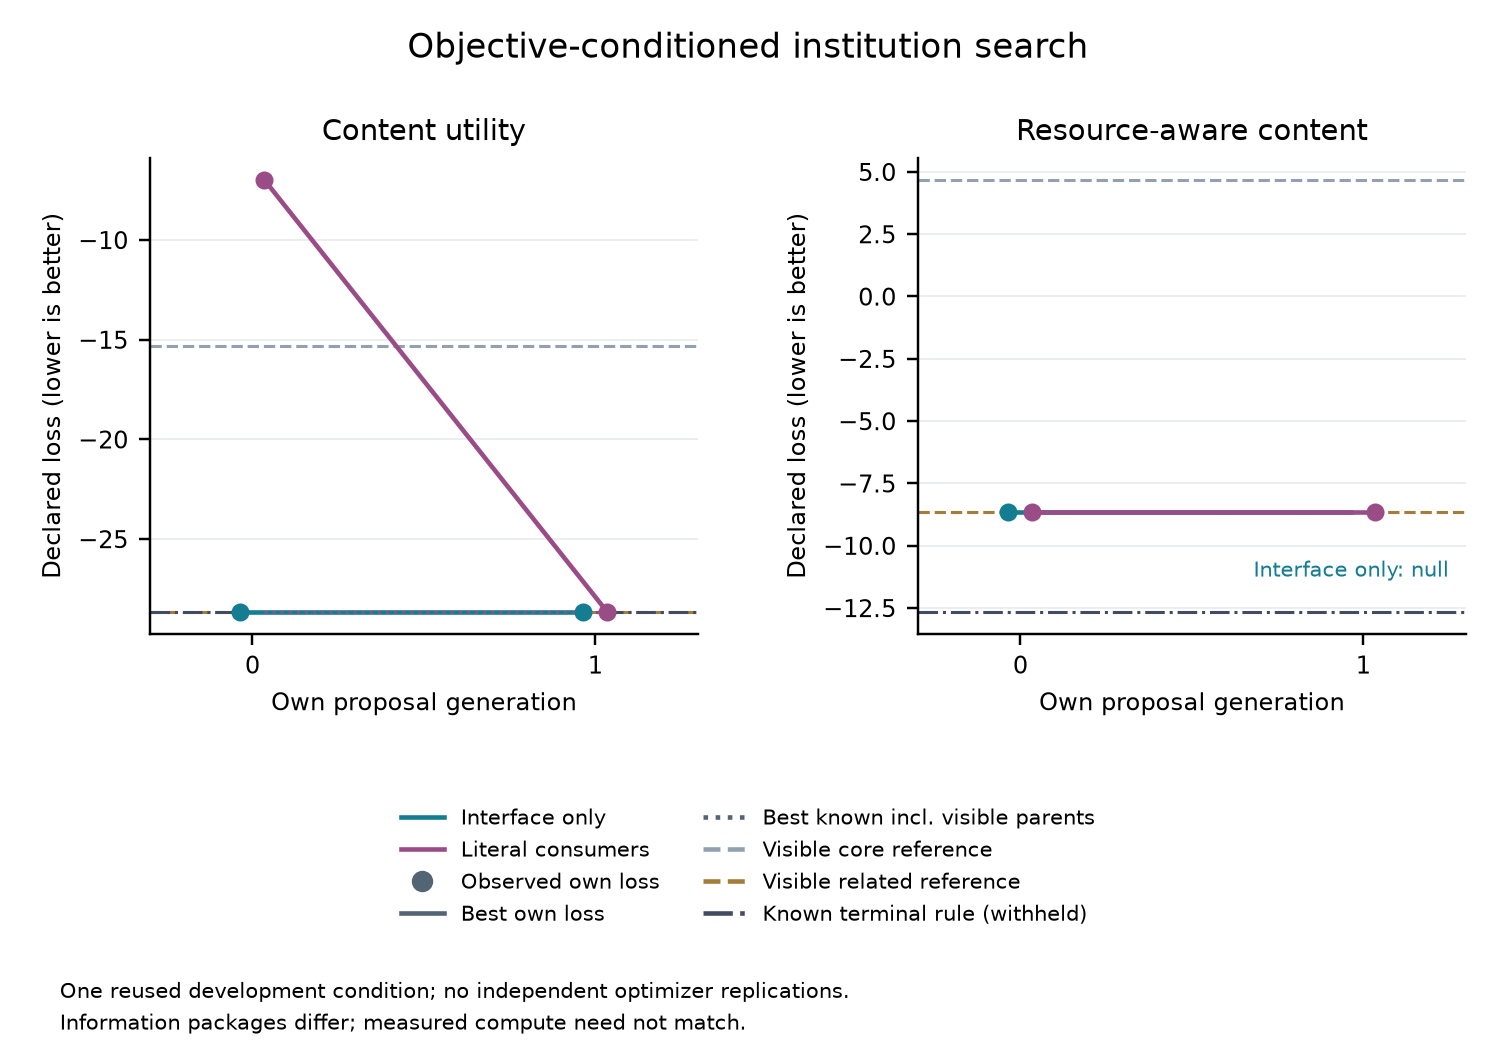
\includegraphics[width=\linewidth]{figures/native-consumer-source-loss-paths-v1.png}
\caption{Four actual search histories under two objectives. Points are observed own
losses; solid paths track best own submission and dotted paths include visible
parents. The adverse source/U path recovers only the known reference. A null
annotation has no numeric vertical meaning, and the incumbent may remain after
failure. The withheld terminal line stays outside both optimizers' parent pools.
One reused condition and unequal information packages do not supply independent
optimizer error bars, isolated comprehension effects or equal measured compute.}
\label{fig:native-consumer-source-paths}
\end{figure}

\subsection{Costs, reconstruction and the next scientific boundary}
The original finite writer exits normally after 17,863.53s (4h57m43.53s) on the
shared local host, not a dedicated machine-speed benchmark. Both original cold
audits and complete cost exports match. The first waiting readout stops at its
existing external-output guard because the launch destination is source-local.
That stopped record remains. A separate read-only export uses the same frozen
reader code, same raw data and matching audit/cost files at a fresh external
destination; both report/CSV/manifest sets then match. No scientist, critic,
proposal, candidate or selection is repeated for this correction.

\begin{table}[t]
\centering\small
\setlength{\tabcolsep}{5pt}
\begin{tabular}{lrrrr}
\toprule
Role & Responses/POSTs & Input tokens & Output tokens & Cached-input subset\\
\midrule
Scientists & 1,650 & 2,395,104 & 153,603 & 358,440\\
Content critics & 198 & 94,806 & 29,111 & ---\\
Designer readiness & 284 & 5,825,760 & 14,027 & 77,500\\
Designer proposals & 101 & 4,018,739 & 26,804 & 212,450\\
Designer loads & 18 & --- & --- & ---\\
Scientist loads & 11 & --- & --- & ---\\
\bottomrule
\end{tabular}
\caption{Separate complete role journals, not a sum of nested timers or
inferred counts from displayed author steps. Missing load usage and unreported
critic cache usage remain unknown. Cached-input counts are subsets, not added
to input totals. The 92 returned component probes make no extra model calls or
native worlds. These computational quantities are separate from native $K$;
FLOPs, energy, monetary cost and dedicated-host speed are not measured.}
\label{tab:native-consumer-source-costs}
\end{table}

All eleven literal submitted/reference systems, frozen selection, cross-scores,
paths and source/hash receipts are retained. Both final seven-file figure
exports match, with inspected layouts; an initial overlapping null annotation
is preserved in its earlier exports and corrected only in presentation.
The observed zero contrast does not demonstrate useful local invention from
this source package. It does not show that source information
never helps, that the reference is optimal or that whole-system design cannot
improve. With only two proposals per history, a reused condition and this local
author/interface, no general method ranking is identified. The next research
decision concerns effective search and strong restricted comparators, not
automatically enlarging a flat result. Important differentiated findings,
appropriate independent histories and selection-frozen unused evaluation
remain necessary; this closed pilot is not main-track readiness.
\FloatBarrier

